% !TeX spellcheck = russian-aot-ieyo
% Зачем: Определяет класс документа (То, как будет выглядеть документ)
% Примечание: параметр draft помечает строки, вышедшие за границы страницы, прямоугольником, в фильной версии его нужно удалить.
\documentclass[a4paper,14pt,russian,oneside,final]{extreport}

% Зачем: Установка кодировки исходных файлов.
\usepackage[utf8]{inputenc}

% Зачем: Делает результирующий PDF "searchable and copyable".
\usepackage{cmap}

% Зачем: Выбор внутренней TeX кодировки.
\usepackage[T2A]{fontenc}

% Зачем: Чтобы можно было использовать русские буквы в формулах, но в случае использования предупреждать об этом.
\usepackage[warn]{mathtext}

% Зачем: Учет особенностей различных языков.
\usepackage[russian]{babel}

% Зачем: Улучшает отображение русских шрифтов.
% Примечание: Требует шаманства при установке, инструкция http://plumbum-blog.blogspot.com/2010/06/miktex-28-pscyr-04d.html
\usepackage{pscyr}


% Зачем: Добавляет поддержу дополнительных размеров текста 8pt, 9pt, 10pt, 11pt, 12pt, 14pt, 17pt, and 20pt.
% Почему: Пункт 2.1.1 Требований по оформлению пояснительной записки.
\usepackage{extsizes}


% Зачем: Длинна, пимерно соответвующая 5 символам
% Почему: Требования содержат странное требование про отсупы в 5 символов (для немоноширинного шрифта :| )
\newlength{\fivecharsapprox}
\setlength{\fivecharsapprox}{6ex}


% Зачем: Добавляет отступы для абзацев.
% Почему: Пункт 2.1.3 Требований по оформлению пояснительной записки.
\usepackage{indentfirst}
\setlength{\parindent}{\fivecharsapprox} % Примерно соответсвует 5 символам.


% Зачем: Настраивает отступы от границ страницы.
% Почему: Пункт 2.1.2 Требований по оформлению пояснительной записки.
\usepackage[left=3cm,top=2.0cm,right=1.5cm,bottom=2.7cm]{geometry}


% Зачем: Настраивает межстрочный интервал, для размещения 40 +/- 3 строки текста на странице.
% Почему: Пункт 2.1.1 Требований по оформлению пояснительной записки.
\usepackage[nodisplayskipstretch]{setspace} 
%\setstretch{1.5}
\onehalfspacing

% Зачем: Выбор шрифта по-умолчанию. 
% Почему: Пункт 2.1.1 Требований по оформлению пояснительной записки.
% Примечание: В требованиях не указан, какой именно шрифт использовать. По традиции используем TNR.
\renewcommand{\rmdefault}{ftm} % Times New Roman


% Зачем: Отключает использование изменяемых межсловных пробелов.
% Почему: Так не принято делать в текстах на русском языке.
\frenchspacing


% Зачем: Сброс счетчика сносок для каждой страницы
% Примечание: в "Требованиях по оформлению пояснительной записки" не указано, как нужно делать, но в других БГУИРовских докуметах рекомендуется нумерация отдельная для каждой страницы
\usepackage{perpage}
\MakePerPage{footnote}


% Зачем: Добавляет скобку 1) к номеру сноски
% Почему: Пункты 2.9.2 и 2.9.1 Требований по оформлению пояснительной записки.
\makeatletter 
\def\@makefnmark{\hbox{\@textsuperscript{\normalfont\@thefnmark)}}}
\makeatother


% Зачем: Расположение сносок внизу страницы
% Почему: Пункт 2.9.2 Требований по оформлению пояснительной записки.
\usepackage[bottom]{footmisc}


% Зачем: Переопределяем стандартную нумерацию, т.к. в отчете будут только section и т.д. в терминологии TeX
\makeatletter
\renewcommand{\thesection}{\arabic{section}}
\makeatother


% Зачем: Пункты (в терминологии требований) в терминологии TeX subsubsection должны нумероваться
% Почему: Пункт 2.2.3 Требований по оформлению пояснительной записки.
\setcounter{secnumdepth}{3}


% Зачем: Настраивает отступ между таблицей с содержанимем и словом СОДЕРЖАНИЕ
% Почему: Пункт 2.2.7 Требований по оформлению пояснительной записки.
\usepackage{tocloft}
\setlength{\cftbeforetoctitleskip}{-1em}
\setlength{\cftaftertoctitleskip}{1em}


% Зачем: Определяет отступы слева для записей в таблице содержания.
% Почему: Пункт 2.2.7 Требований по оформлению пояснительной записки.
\makeatletter
\renewcommand{\l@section}{\@dottedtocline{1}{0.5em}{1.2em}}
\renewcommand{\l@subsection}{\@dottedtocline{2}{1.7em}{2.0em}}
\makeatother


% Зачем: Работа с колонтитулами
\usepackage{fancyhdr} % пакет для установки колонтитулов
\pagestyle{fancy} % смена стиля оформления страниц


% Зачем: Нумерация страниц располагается справа снизу страницы
% Почему: Пункт 2.2.8 Требований по оформлению пояснительной записки.
\fancyhf{} % очистка текущих значений
\fancyfoot[R]{\thepage} % установка верхнего колонтитула
\renewcommand{\footrulewidth}{0pt} % убрать разделительную линию внизу страницы
\renewcommand{\headrulewidth}{0pt} % убрать разделительную линию вверху страницы
\fancypagestyle{plain}{ 
    \fancyhf{}
    \rfoot{\thepage}}


% Зачем: Задает стиль заголовков раздела жирным шрифтом, прописными буквами, без точки в конце
% Почему: Пункты 2.1.1, 2.2.5, 2.2.6 и ПРИЛОЖЕНИЕ Л Требований по оформлению пояснительной записки.
\makeatletter
\renewcommand\section{%
  \clearpage\@startsection {section}{1}%
    {\fivecharsapprox}%
    {-1em \@plus -1ex \@minus -.2ex}%
    {1em \@plus .2ex}%
    {\raggedright\hyphenpenalty=10000\normalfont\large\bfseries\MakeUppercase}}
\makeatother


% Зачем: Задает стиль заголовков подразделов
% Почему: Пункты 2.1.1, 2.2.5 и ПРИЛОЖЕНИЕ Л Требований по оформлению пояснительной записки.
\makeatletter
\renewcommand\subsection{%
  \@startsection{subsection}{2}%
    {\fivecharsapprox}%
    {-1em \@plus -1ex \@minus -.2ex}%
    {1em \@plus .2ex}%
    {\raggedright\hyphenpenalty=10000\normalfont\normalsize\bfseries}}
\makeatother


% Зачем: Задает стиль заголовков пунктов
% Почему: Пункты 2.1.1, 2.2.5 и ПРИЛОЖЕНИЕ Л Требований по оформлению пояснительной записки.
\makeatletter
\renewcommand\subsubsection{
  \@startsection{subsubsection}{3}%
    {\fivecharsapprox}%
    {-1em \@plus -1ex \@minus -.2ex}%
    {\z@}%
    {\raggedright\hyphenpenalty=10000\normalfont\normalsize\bfseries}}
\makeatother

% Зачем: для оформления введения и заключения, они должны быть выровнены по центру.
% Почему: Пункты 1.1.15 и 1.1.11 Требований по оформлению пояснительной записки.
\makeatletter
\newcommand\sectioncentered{%
  \clearpage\@startsection {section}{1}%
    {\z@}%
    {-1em \@plus -1ex \@minus -.2ex}%
    {1em \@plus .2ex}%
    {\centering\hyphenpenalty=10000\normalfont\large\bfseries\MakeUppercase}%
    }
\makeatother



% Зачем: Задает стиль библиографии
% Почему: Пункт 2.8.6 Требований по оформлению пояснительной записки.
\bibliographystyle{styles/belarus-specific-utf8gost780u}


% Зачем: Пакет для вставки картинок
% Примечание: Объяснение, зачем final - http://tex.stackexchange.com/questions/11004/why-does-the-image-not-appear
\usepackage[final]{graphicx}
\DeclareGraphicsExtensions{.pdf,.png,.jpg,.eps}


% Зачем: Директория в которой будет происходить поиск картинок
\graphicspath{{figures/}}


% Зачем: Добавление подписей к рисункам
\usepackage[nooneline]{caption}
\usepackage{subcaption}

% Зачем: Задание подписей, разделителя и нумерации частей рисунков
% Почему: Пункт 2.5.5 Требований по оформлению пояснительной записки.
\DeclareCaptionLabelFormat{stbfigure}{Рисунок #2}
\DeclareCaptionLabelFormat{stbtable}{Таблица #2}
\DeclareCaptionLabelSeparator{stb}{~--~}
\captionsetup{labelsep=stb}
\captionsetup[figure]{labelformat=stbfigure,justification=centering}
\captionsetup[table]{labelformat=stbtable,justification=raggedright}
\renewcommand{\thesubfigure}{\asbuk{subfigure}}

% Зачем: Окружения для оформления формул
% Почему: Пункт 2.4.7 требований по оформлению пояснительной записки и специфические требования различных кафедр
\usepackage{tabularx}

\newenvironment{explanation}
    {
    %%% Следующие строки определяют специфические требования кафедр. Раскоменнтируйте нужные 2 строки
    %% стандартный абзац, Кафедра информатики
    \par 
    \tabularx{\textwidth-\fivecharsapprox}{@{}ll@{ --- } X }
    %% без отступа, Кафедра экономической информатики
    %\noindent 
    %\tabularx{\textwidth}{@{}ll@{ --- } X }
    }
    { 
    \\[\parsep]
    \endtabularx
    }


% Зачем: Удобная вёрстка многострочных формул, масштабирующийся текст в формулах, формулы в рамках и др
\usepackage{amsmath}


% Зачем: Поддержка ажурного и готического шрифтов 
\usepackage{amsfonts}


% Зачем: amsfonts + несколько сотен дополнительных математических символов
\usepackage{amssymb}


% Зачем: Окружения «теорема», «лемма»
\usepackage{amsthm}


% Зачем: Производить арифметические операции во время компиляции TeX файла
\usepackage{calc}

% Зачем: Производить арифметические операции во время компиляции TeX файла
\usepackage{fp}

% Зачем: Пакет для работы с перечислениями
\usepackage{enumitem}
\makeatletter
 \AddEnumerateCounter{\asbuk}{\@asbuk}{щ)}
\makeatother


% Зачем: Устанавливает символ начала простого перечисления
% Почему: Пункт 2.3.5 Требований по оформлению пояснительной записки.
\setlist{nolistsep}


% Зачем: Устанавливает символ начала именованного перечисления
% Почему: Пункт 2.3.8 Требований по оформлению пояснительной записки.
\renewcommand{\labelenumi}{\asbuk{enumi})}
\renewcommand{\labelenumii}{\arabic{enumii})}

% Зачем: Устанавливает отступ от границы документа до символа списка, чтобы этот отступ равнялся отступу параграфа
% Почему: Пункт 2.3.5 Требований по оформлению пояснительной записки.

\setlist[itemize,0]{itemindent=\parindent + 2.2ex,leftmargin=0ex,label=--}
\setlist[enumerate,1]{itemindent=\parindent + 2.7ex,leftmargin=0ex}
\setlist[enumerate,2]{itemindent=\parindent + \parindent - 2.7ex}

% Зачем: Включение номера раздела в номер формулы. Нумерация формул внутри раздела.
\AtBeginDocument{\numberwithin{equation}{section}}

% Зачем: Включение номера раздела в номер таблицы. Нумерация таблиц внутри раздела.
\AtBeginDocument{\numberwithin{table}{section}}

% Зачем: Включение номера раздела в номер рисунка. Нумерация рисунков внутри раздела.
\AtBeginDocument{\numberwithin{figure}{section}}


% Зачем: Дополнительные возможности в форматировании таблиц
\usepackage{makecell}
\usepackage{multirow}
\usepackage{array}


% Зачем: "Умная" запятая в математических формулах. В дробных числах не добавляет пробел
% Почему: В требованиях не нашел, но в русском языке для дробных чисел используется {,} а не {.}
\usepackage{icomma}

% Зачем: макрос для печати римских чисел
\makeatletter
\newcommand{\rmnum}[1]{\romannumeral #1}
\newcommand{\Rmnum}[1]{\expandafter\@slowromancap\romannumeral #1@}
\makeatother


% Зачем: Управление выводом чисел.
\usepackage{sistyle}
\SIdecimalsign{,}

% Зачем: inline-коментирование содержимого.
\newcommand{\ignore}[2]{\hspace{0in}#2}


% Зачем: Возможность коментировать большие участки документа
\usepackage{verbatim}


\usepackage{xcolor}


% Зачем: Оформление листингов кода
% Примечание: final нужен для переопределения режима draft, в котором листинги не выводятся в документ.
\usepackage[final]{listings}


% Зачем: настройка оформления листинга для языка F#
\definecolor{bluekeywords}{rgb}{0.13,0.13,1}
\definecolor{greencomments}{rgb}{0,0.5,0}
\definecolor{turqusnumbers}{rgb}{0.17,0.57,0.69}
\definecolor{redstrings}{rgb}{0.5,0,0}

\renewcommand{\lstlistingname}{Листинг}

\lstdefinelanguage{FSharp}
    {morekeywords={abstract,and,as,assert,base,begin,class,default,delegate,do,done,downcast,downto,elif,else,end,exception,extern,false,finally,for,fun,function,global,if,in,inherit,inline,interface,internal,lazy,let,let!,match,member,module,mutable,namespace,new,not,null,of,open,or,override,private,public,rec,return,return!,select,static,struct,then,to,true,try,type,upcast,use,use!,val,void,when,while,with,yield,yield!,asr,land,lor,lsl,lsr,lxor,mod,sig,atomic,break,checked,component,const,constraint,constructor,continue,eager,event,external,fixed,functor,include,method,mixin,object,parallel,process,protected,pure,sealed,tailcall,trait,virtual,volatile},
    keywordstyle=\bfseries\color{bluekeywords},
    sensitive=false,
    morecomment=[l][\color{greencomments}]{///},
    morecomment=[l][\color{greencomments}]{//},
    morecomment=[s][\color{greencomments}]{{(*}{*)}},
    morestring=[b]",
    stringstyle=\color{redstrings},
    }

\lstdefinestyle{fsharpstyle}{
   xleftmargin=0ex,
   language=FSharp,
   basicstyle=\footnotesize\ttfamily,
   breaklines=true,
   columns=fullflexible
}

\lstdefinestyle{csharpinlinestyle} {
  language=[Sharp]C,
  morekeywords={yield,var,get,set,from,select,partial,where,async,await},
  breaklines=true,
  columns=fullflexible,
  basicstyle=\footnotesize\ttfamily
}

\lstdefinestyle{csharpstyle}{
  language=[Sharp]C,
  frame=lr,
  rulecolor=\color{blue!80!black}}


% Зачем: Нумерация листингов в пределах секции
\AtBeginDocument{\numberwithin{lstlisting}{section}}

\usepackage[normalem]{ulem}

\usepackage[final]{hyperref}
% Моноширинный шрифт выглядит визуально больше, чем пропорциональный шрифт, если их размеры одинаковы. Искусственно уменьшаем размер ссылок.
\renewcommand{\UrlFont}{\small\rmfamily\tt}

\usepackage[square,numbers,sort&compress]{natbib}
\setlength{\bibsep}{0em}

% Магия для подсчета разнообразных объектов в документе
\usepackage{lastpage}
\usepackage{totcount}
\regtotcounter{section}

\usepackage{etoolbox}

\newcounter{totfigures}
\newcounter{tottables}
\newcounter{totreferences}
\newcounter{totequation}

\providecommand\totfig{} 
\providecommand\tottab{}
\providecommand\totref{}
\providecommand\toteq{}

\makeatletter
\AtEndDocument{%
  \addtocounter{totfigures}{\value{figure}}%
  \addtocounter{tottables}{\value{table}}%
  \addtocounter{totequation}{\value{equation}}
  \immediate\write\@mainaux{%
    \string\gdef\string\totfig{\number\value{totfigures}}%
    \string\gdef\string\tottab{\number\value{tottables}}%
    \string\gdef\string\totref{\number\value{totreferences}}%
    \string\gdef\string\toteq{\number\value{totequation}}%
  }%
}
\makeatother

\pretocmd{\section}{\addtocounter{totfigures}{\value{figure}}\setcounter{figure}{0}}{}{}
\pretocmd{\section}{\addtocounter{tottables}{\value{table}}\setcounter{table}{0}}{}{}
\pretocmd{\section}{\addtocounter{totequation}{\value{equation}}\setcounter{equation}{0}}{}{}
\pretocmd{\bibitem}{\addtocounter{totreferences}{1}}{}{}

\newcommand{\specialcell}[2][c]{%
  \begin{tabular}[#1]{@{}c@{}}#2\end{tabular}}


% Для оформления таблиц не влязящих на 1 страницу
\usepackage{longtable}
\usepackage{makecell}

% Для включения pdf документов в результирующий файл
\usepackage{pdfpages}


\input{macro_glob}

\begin{document}

%\input{diploma_title} % page 1

% \input{abstract} % page 2

% \input{diploma_task} % pages 3 and 4. printed separately

% \input{annotation} % not part of report

%\input{feedback} % not part of report

%\input{review} % not part of report

\setcounter{page}{3}

\input{table_of_contents}

\sectioncentered*{Введение}
\addcontentsline{toc}{section}{Введение}
\label{sec:intro}

Экспоненциальный рост ресурсов сети Интернет
сделал обыденным
потоковую передачу видеотрафика в режиме реального времени.
В настоящее время организация видеозвонков и видеоконференций
на базе интернет-сервисов, подобных Skype\footnote{\texttt{\url{http://skype.com}}} и
GoogleTalk\footnote{\texttt{\url{http://www.google.com/hangouts/}}} является повсеместной практикой.
Заинтересованность крупных корпораций в программном
обеспечении телеконференций и удалённых совещаний
привела к созданию многочисленных коммерческих продуктов
по передаче видео по сети Интернет, таким, как
WebEx\footnote{\texttt{\url{http://www.webex.com/}}}
и Adobe Connect\footnote{\texttt{\url{http://www.webex.com/}}}
Подобные программные решения
существенно поднимают планку требований к характеристикам
качества обслуживания, предъявляемых к сетям передачи
данных. Приведённые соображения свидетельствуют и о
необходимости в целенаправленном развитии мультимедиа-сетевых
технологий.

Одним из основных составляющих мультимедиа-сетевых технологий
является сжатие данных, или кодирование источника~\cite{salomoncomp, sklarbook}
в терминах теории информации, задачей которого является
уменьшение избыточности мультимедиа источника (аудио,
видео или изображения). Сжатие видео -- это процедура,
позволяющая уменьшить объём информации, необходимый
для представления цифрового видеосигнала, предшествующая передаче
этого сигнала по сети или сохранения на электронном носителе.
В рамках стека мультимедиа-сетевых технологий сжатые данные
передаются по сети Интернет.

Контроль битовой скорости (англ. bit-rate control) является
важнейшим элементом большей части видеокодеров. Этот
компонент определяет количество бит, затрачиваемых на один
кадр и его качество. Существуют два типа контроля битовой
скорости выхода видеокодера: ориентирование на постоянную
(англ. constant bit-rate) и переменную (англ. variable bit-rate, VBR)
битовые скорости. При постоянной битовой скорости задачей
видеокодера является оптимизация качества передаваемого
видео при максимальном приближении размера сжатого кадра
к требуемому~\cite{survey2013}. Это приводит к колебаниям качества
при смене сцен, освещения и сценах с повышенным
движением в кадре. Видеокодеры с переменной битовой
скоростью используются при необходимости поддерживать постоянное
качество видеосигнала и при смягчённых требованиях
передачи видеотрафика в реальном времени.

В данной работе рассматривается моделирование
сжатого видеотрафика с переменной битовой скоростью.

Моделирование видеотрафика позволяет контролировать
пригодность сети для использования в качестве транспорта
при передаче видео на этапе её проектирования,
а также использовать искусственно сгенерированный трафик
при нагрузочном тестировании существующей сети.

В литературе было предложено большое количество моделей
видеотрафика, адаптированных под видеоданные разной природы.
В данной работе описаны основные подходы к классификации
и моделированию видеотрафика. Проанализированы особенности
конкретного типа видеотрафика --- трафика видеоконференций
--- для которого реализованы две модели:
дискретно-авторегрессионная и марковская. Для марковской
модели предложена и реализована оптимизация, позволяющая
уменьшить количество ``вырожденных'' состояний.

Вопрос сравнения различных моделей остаётся открытым:
модели видеотрафика часто базируются на совершенно
различных математических аппаратах и принципах.
Какие критерии позволят сделать вывод о превосходстве
одной модели над другими? В данной дипломной работе
рассмотрены основные методы сравнения моделей и
предложен дополнительный метод сравнения моделей
на основе оценки задержки и джиттера.

Осуществлён сравнительный анализ реализованных моделей
для стандартных тестовых видео базы Государственного
Университета Аризоны~\cite{traceas}, которая используется
специалистами в области обработки мультимедиа в качестве
``общего знаменателя'', и для самостоятельно записанных
видео подходящего типа, необходимость в которых объясняется
отсутствием в базе тестовых видео требуемой длительности
в широком спектре разрешений.

\section{Обзор предметной области}
\label{sec:survey}
\subsection{Постановка задачи моделирования видеотрафика
с переменной битовой скоростью}

Пусть есть некоторая видеопоследовательность ---
последовательность изображений в цифровом RAW-формате.
Данная последовательность подвергается сжатию с помощью
некоторого видеокодера, сконфигурированного с целью
сохранения качества видео при переменном размере кадра.

В данной работе в качестве стандарта видеокодера
используется H.264~\cite{h264spec}, один из распространённых
стандартов сжатия видео. Кадровая частота, размер кадров (разрешение)
и цветовое разрешение тестовой последовательности известны.

С точки зрения моделирования видеотрафика, сжатый видеопоток
можно представить как последовательность из $N$ кадров
размера $S_i,~i=1\dots N$. Внутренняя структура сжатого
кадра не рассматривается. Кадры, тем не менее, разделены
на три типа в зависимости от использования и типе межкадрового
предсказания (англ. inter-frame prediction)~\cite{salomoncomp}.
В стандарте H.264~\cite{h264spec} предусмотрено разбиение каждого
кадра на прямоугольные области одинакового размера (макроблоки),
для каждой из которых индивидуально определяется тип и наличие
предсказания, но с ограничением, определяемым типом всего кадра:

\begin{itemize}
    \item I-кадры (также называются ``ключевыми'', англ. intra-frames).
        Содержат только макроблоки, сжатые независимо от макроблоков
        других кадров.
    \item P-кадры (``разностные'' кадры, англ. predicted frames).
        Могут содержать как макроблоки, сжатые независимо от других
        кадров, так и макроблоки, сжатие которых осуществлялось с
        опорой на другой предшествующий I- или P-кадр.
    \item B-кадры (``двунаправленные'' кадры, англ. bi-predicted frames).
        Могут содержать макроблоки следующих типов: предсказанные с опорой
        на другой I-, P-, B-кадры или с опорой на два кадра любого в
        общем случае типа, один из которых предшествует текущему,
        а другой следует за текущим кадром.
\end{itemize}

Как правило, в видеокодеках используется некоторая техника
разностной импульсно-кодовой модуляции (англ. differential
pulse-code modulation, DPCM)~\cite{sklarbook}, предполагающая некоторую
процедуру предсказания текущего макроблока по множеству других.
Выбор макроблоков, на основе которых производить предсказание,
и является критерием типизации макроблоков и кадров.

Наличие ``опорных'' кадров позволяет существенно ускорить
время получения произвольного кадра в потоке и ``быстрой
перемотки с показом'', поскольку в этом случае декодирование
можно начинать с ближайшего ``опорного'' I-кадра.
Однако предсказание лишь на основе текущего кадра не
позволяет использовать временн\'{у}ю избыточность
видеопотока~\cite{salomoncomp}.

``Разностные'' кадры позволяют
экстраполировать временн\'{о}е поведение видеопотока
и получить более точное предсказание. ``Двусторонние''
кадры заменяют временн\'{у}ю экстраполяцию интерполяцией,
что приводит к повышению точности предсказания.
Использование межкадрового предсказания требует
усложнения процедуры декодирования ввиду необходимости в
буферизации как декодированных (I- и P-кадры), так и
сжатых кадров (для использования двустороннего предсказания).

Цепочки кадров разных типов между соседними I-кадрами называются
GOP (англ. Group of Pictures). Типовая цепочка, используемая
в кодеком x264 (реализацией стандарта H.264)~\cite{x264page},
имеет вид

$$
\mathtt{IBBPBBPBBPBBPBBPBBPBBPBBP}.
$$

В ней B-кадры
ссылаются на два ближайших I- или P-кадра и независимы
между собой. Данная структура схематически изображена
на Рис.~\ref{fig:ipb_frames}.

\begin{figure}[h]
    \begin{center}
        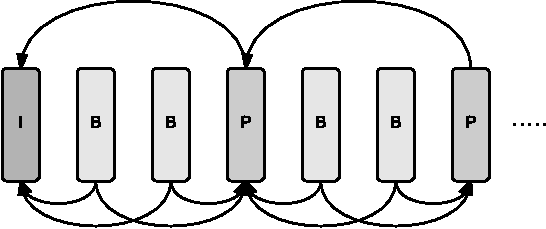
\includegraphics[width=0.7\textwidth]{ipb_chart.pdf}
    \end{center}
    \caption{Схематическое изображение структуры сжатого потока
    для кодека x264 по умолчанию}
    \label{fig:ipb_frames}
\end{figure}

Значительная часть моделей видеотрафика~\cite{survey2013} разделяют
сжатый поток кадров разного типа на подпотоки и моделируют
их независимо, получая результирующий поток путём последующего
совмещения подпотоков в соответствии с требуемой схемой.
При таком подходе основной задачей моделирования является
моделирование подпотока одного типа.

В данной работе рассматривается задача моделирования потока
P-кадров, в котором каждый последующий кадр ссылается на
предыдущий. Схема данного потока проиллюстрирована на Рис.~\ref{fig:ippp_frames}.

\begin{figure}[h]
    \begin{center}
        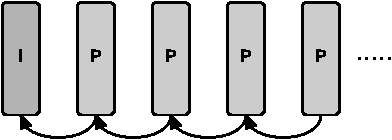
\includegraphics[width=0.55\textwidth]{ippp_chart.pdf}
    \end{center}
    \caption{Схематическое изображение моделируемой структуры сжатого потока
    для кодека x264}
    \label{fig:ippp_frames}
\end{figure}

Таким образом, в задачи данного дипломного проекта входит:

\begin{itemize}
    \item анализ особенностей сжатого VBR-трафика видеоконференций;
    \item обзор существующих моделей VBR-видеотрафика и анализ
        целесообразности их использования при моделировании
        трафика видеоконференций;
    \item реализация набора существующих моделей VBR-видеотрафика
        и методики их адаптации к особенностям трафика видеоконференций;
    \item обзор методов сравнительного анализа моделей;
    \item сравнительный анализ результатов моделирования VBR-трафика
        видеоконференций.
\end{itemize}

\subsubsection{Формальное определение задачи}
\label{sse:task}
\hspace{3pt}

Приведённые ограничения позволяют предложить формальное определение задачи
моделирования выхода видеокодера с переменной битовой скоростью.
Пусть $S = \{S_i\} _{i=1}^N$ --- последовательность размеров P-кадров на выходе видеокодера.
$S$ можно рассматривать как реализацию случайного процесса $\Sigma$~\cite{randomprocesses}
\begin{itemize}
    \item с дискретными состояниями (размеры кадров)
    \item дискретного по времени ($\tau$ -- интервал следования кадров -- единица измерения времени)
    \item неизвестной структуры
\end{itemize}

Задача моделирования видеокодера может быть сформулирована в терминах
теории о вероятностных процессах как определение случайного
процесса $\Sigma$ по набору его реализаций $S$.

Эта задача не имеет решения, поэтому исследователи видеотрафика
прибегают~\cite{characteristics2013} к эвристическим методам определения структуры
случайного процесса. Задача моделирования видеотрафика может быть
сформулирована следующим образом: предложить случайный процесс
$\Sigma'(S)$, реализации $S'$ которого будут ``соответствовать''
реализации $S$ по набору характеристик. Таким образом,
каждая тестовая видеопоследовательность рассматривается
как реализация случайного процесса, которая используется
для ``адаптации'' модели $\Sigma'$ под особенности
конкретного видео.

\subsection{Анализ особенностей трафика видеоконференций}
%\hspace{3pt}

С точки зрения специалистов в области сжатия видео~\cite{survey2013},
видеоданные могут быть условно разделены на классы по
следующим параметрам:

\begin{itemize}
    \item ``активность'' (количество движения) в кадре. Численно 
        эту характеристику можно оценить путём получения разности
        двух последовательных кадров;
    \item ``локальность'' движения. Сосредоточенность энергии
        разностного кадра в конкретных областях кадра;
    \item наличие ``смены сцен''. Смена сцены --- это эвристически
        определяемая резкая перемена освещения, смена плана,
        и тому подобное. Обычно определяется~\cite{scenedetection} как превышение
        энергии разностного кадра некоторого порога;
    \item геометрические размеры кадра (разрешение)
    \item зашумлённость
    \item требования к качеству сжатого видео: глубина цвета,
        разрешение, соотношение сигнал-шум (PSNR)~\cite{salomoncomp}.
\end{itemize}

Обычно видео разделяют на подтипы по происхождению,
каждый из которых обладает собственным набором признаков.
Для видеопоследовательностей разных классов требуются
различные конфигурации видеокодека или даже разработка
собственного кодека, приспособленного под данный класс видео.

\begin{table}[ht]
    \caption{Сравнение отличительных особенностей несжатого видеотрафика разного происхождения}
    \centering
    \begin{tabular}{| c | c | c | c | c | c |}
\hline
                      & Спорт    & CCTV     & Conference  & Кино       & Casual  \\
\hline
\specialcell{Активность\\в кадре}    &  Высокая &  Малая   &  Малая      & Переменная & Высокая \\
\hline
\specialcell{Локальность\\движения}  &  Низкая  &  Высокая &  Высокая    & Переменная & Низкая  \\
\hline
Зашумлённость         &  Низкая  &  Высокая &  Переменная & Низкая     & Высокая \\
\hline
Смена сцен            &  Частая  &  Редкая  &  Отсутствие & Частая     & Частая  \\
\hline
    \end{tabular}
    \label{tab:videotypes}
\end{table}

В данной дипломной работе объектом моделирования является
сжатый трафик видеоконференций, который в несжатом виде
характеризуется следующими признаками (Таблица~\ref{tab:videotypes}):

\begin{itemize}
    \item малая активность в кадре;
    \item локальный характер движения;
    \item отсутствие смены сцен;
    \item умеренная зашумлённость.
\end{itemize}

\subsection{Использованное при моделировании тестовое множество}
%\hspace{3pt}

Вышеприведённые особенности несжатого трафика видеоконференций
были критерием отбора тестовых видео. Тестовое множество было
составлено из десяти видеозаписей, половина из которых
находилась в базе тестовых видео Государственного Университета
Аризоны~\cite{traceas}, которая используется специалистами в области
сжатия видео в качестве ``общего знаменателя'', который позволяет
сравнивать различные алгоритмы сжатия видео на одинаковых
видеопоследовательностях. Следующие видеозаписи были
признаны подходящими для использования в качестве
записей видеоконференций:

\begin{itemize}
    \item Akiyo
    \item Foreman
    \item Miss-America
    \item Suzie
    \item Claire
\end{itemize}

Данные видеозаписи имеют низкое разрешение (примерно 300x300 пикселей)
и маленькую продолжительность (примерно 300-500 кадров при кадровой
скорости 25 кадров в секунду). С помощью встроенной веб-камеры были
самостоятельно получены более продолжительные тестовые видеопоследовательности
различного разрешения и качества:

\begin{itemize}
    \item Boris
    \item RomanL
    \item RomanM
    \item RomanS
    \item RomanSQ
\end{itemize}

\begin{table}[ht]
\caption{Характеристики тестового множества}
\centering
\begin{tabular}{| c | c | c | c | c |}
\hline
              & Разрешение & Длительность & FPS & QP \\ \hline
Akiyo         & 176x144    & 12s          & 25  & 5  \\ \hline
Foreman       & 176x144    & 12s          & 25  & 5  \\ \hline
Miss-America  & 176x144    & 6s           & 25  & 5  \\ \hline
Suzie         & 176x144    & 6s           & 25  & 5  \\ \hline
Claire        & 176x144    & 20s          & 25  & 5  \\ \hline
Boris         & 480x320    & 2h           & 30  & 11 \\ \hline
RomanL        & 1280x720   & 10m          & 30  & 5  \\ \hline
RomanM        & 640x480    & 20m          & 30  & 5  \\ \hline
RomanS        & 320x240    & 10m          & 30  & 5  \\ \hline
RomanSQ       & 320x240    & 10m          & 30  & 25 \\ \hline
\end{tabular}
\label{tab:videos}
\end{table}

Характеристики сжатого видео представлены в таблице~\ref{tab:videos}.
В данной таблице используются следующие обозначения:
\begin{itemize}
    \item QP (англ. Quantization Parameter) --- это параметр кодера x264,
        значение которого прямо пропорционально степени сжатия исходного видео
        и, соответственно, обратно пропорционально качеству декодированного;
    \item FPS (англ. Frames Per Second) --- кадровая скорость видео. Период
        следования кадров есть величина, обратная FPS.
\end{itemize}


\subsection{Критерии сравнительного анализа моделей}
%\hspace{3pt}

Формулировка задачи (раздел~\ref{sse:task}) предусматривает
сравнение тестовой видеопоследовательности с синтезированной.
Сравнение последовательностей (трейсов, англ. trace) осуществляется
по тем параметрам, которые играют значение при непосредственной
передаче трафика по сети. Можно выделить две группы сравнительных
характеристик: статистические характеристики и характеристики качества
обслуживания.

Из статистических характеристик интерес представляет распределение
размеров кадров и автокорреляционная структура случайного процесса.

При определении моментов распределения размеров кадров усреденение
по статистическому ансамблю реализаций заменяется на усреднение
по времени. Таким образом, неявно предполагается эргодическая
структура случайного процесса~\cite{ergodic}.

Сравнение характеристик качества обслуживания основывается
на предположении, что точная модель должна демонстрировать
такие же показатели синтетического трейса при передаче по
сети, что и исходная последовательность.

В данной работе следующие характеристики видеопоследовательностей
используются для сравнения тестовых видеопоследовательностей
со сгенерированными:

\begin{itemize}
    \item Статистические характеристики
        \begin{itemize}
            \item гистограмма размеров кадров
            \item первые два момента распределения размеров кадров
            \item автокорреляционная функция последовательности размеров кадров
        \end{itemize}

    \item Характеристики качества обслуживания
        \begin{itemize}
            \item потери при переполнении буфера
            \item задержка
            \item джиттер
        \end{itemize}
\end{itemize}

В разделе~\ref{sec:modelcomp} подробно описана
методика сравнительного анализа моделей на основе
вышеприведённых критериев.

\subsection{Особенности сжатого видеотрафика}
\label{sse:traces}
%\hspace{3pt}

Первым шагом к моделированию сжатого видеотрафика конкретного
типа является исследование его статистических особенностей.
В ходе данного исследования было установлено, что типовая
гистограмма распределения размеров кадров имеет
куполообразный характер. Типовая гистограмма приведена на
рисунке~\ref{fig:romanbell}.

\begin{figure}[h]
    \begin{center}
        \includegraphics[width=\textwidth]{roman_bell.pdf}
    \end{center}
    \caption{Типовая гистограмма распределения размеров кадров (для видео RomanS)}
    \label{fig:romanbell}
\end{figure}

Подобный характер зависимости позволяет аппроксимировать
распределение размеров кадров хорошо изученными аналитическими
распределениями, способными малым числом параметров описывать
большое количество тестовых видеопоследовательностей.
В исследовательских публикациях в таком качестве используется
Гамма-распределение~\cite{heymansourcemodels},
распределение Пирсона типа V~\cite{lazarismodelling},
логарифмическое нормальное распределение~\cite{Krunz95atraffic} и
отрицательное биномиальное распределение~\cite{heymanATM}.

Второй обнаруженной особенностью исследуемого типа видеотрафика
является зависимость автокорреляционной структуры видеопоследовательности
от разрешения и степени квантования видео. В соответствии с рисунком~\ref{fig:acfs},
скорость убывания функции автокорреляции обратно пропорциональна качеству
видеопоследовательности. Природа данного феномена остаётся невыясненной;
коэффициент автокорреляции последовательности инвариантен к её произведению на скаляр,
поэтому меньший размер сжатого кадра как таковой не может являться
причиной изменения функции автокорреляции.

\begin{figure}[h]
    \begin{center}
        \includegraphics[width=\textwidth]{acfs_resolution.pdf}
    \end{center}
    \caption{Автокорреляционная функция для видео разного качества}
    \label{fig:acfs}
\end{figure}

В целом в научных публикациях~\cite{raey} утверждается, функция автокорреляции
для трафика видеоконференций хорошо аппроксисмируется экспонентой. Настоящая
работа готова подтвердить этот результат для видео плохого качества,
но не для высококачественного трафика видеоконференций. На текущий момент
качество (разрешение, степень квантования) передаваемого трафика исследуемого типа
остаётся низким. Однако необходимость в моделировании трафика видеоконференций
высокого качества может привести к разработке моделей с неэкспоненциальной
автокорреляционной структурой.

\newpage
\subsection{Описание существующих подходов к моделированию VBR-видеотрафика}
\label{sse:survey}

В данном подразделе приведено краткое описание основных подходов
к моделированию видеотрафика, описаны их особенности и степень
применимости к моделированию конкретного подкласса видеотрафика ---
трафика видеоконференций.

``Хорошая'' модель видеотрафика должна отражать его статистические
характеристики и демонстрировать такие же характеристики качества
обслуживания при передаче по сети произвольной конфигурации.
Одним из наиболее важных статистических характеристик
видеотрафика является функция автокорреляции (англ. autocorrelation function, ACF)
размеров кадров.
Точное отражение автокорреляционных характеристик видеотрафика ---
сложная задача, потому что в общем случае видеопоследовательности
имеют как краткосрочные (англ. Short-Range Dependent, SRD), так
и долгосрочные (англ. Long-Range Dependent, LRD) зависимости.
С точки зрения автокорреляционной структуры, случайные процессы
могут быть разделены на три типа: независимые, SRD- и LRD-процессы.
У независимых процессов автокорреляция равна нулю при любом
ненулевом смещении. Функция автокорреляции SRD-процессов
убывает экспоненциально. ACF LRD-процессов убывает медленнее~\cite{raey}.

Существующие подходы к моделированию видеотрафика можно условно
разделить на пять классов~\cite{survey2013}:

\begin{itemize}
    \item Авторегрессионные модели: очередной размер кадра
        определяется некоторой функцией от предыдущих кадров
        некоторого временн\'{о}го окна;
    \item Модели, основанные на марковских процессах: марковские
        процессы используются для представления изменений
        в битовой скорости, размеров кадров, сцен или GOP-ов
        (англ. Group of Pictures);
    \item Самоподобные и дробные ARIMA модели: способны отражать
        долгосрочные зависимости в моделируемом трафике;
    \item Вейвлетные модели: вейвлетные преобразования используются
        для того, чтобы отражать как краткосрочные, так и долгосрочные
        зависимости в моделируемом трафике;
    \item Прочие модели: немногочисленные не принадлежащие к
        приведённым классам модели, такие, как модель M/G/$\infty$
        и TES-модель.
\end{itemize}
\hspace{5pt}

Далее приведена краткая характеристика каждого из подходов.

\subsubsection{Авторегрессионные модели}
\hspace{3pt}

Особенностью авторегрессионных случайных процессов является
явная зависимость очередного элемента реализации от фиксированного
количества предыдущих значений. Простой авторегрессионный процесс может
быть описан следующим образом~\cite{ars2004, survey2013}:

\begin{equation}
    S_i = \sum_{k=1}^p a_k S_{i - k} + e_i,
\end{equation}

где $p$ -- порядок авторегрессионного процесса, $a_1, a_2, \dots a_p$ -- коэффициенты
авторегрессии. Последовательность $e_i$ состоит из независимых, равномерно
распределённых случайных величин, которая иногда называется остаточным процессом.
Таким образом, каждый последующий элемент в простом авторегрессионном процессе
есть взвешенная сумма $p$ предыдущих элементов и случайного остатка, в качестве
которого часто используют аддитивный белый гауссовский шум (АБГШ) с нулевым средним
и оценённым на основе тестовой последовательности дисперсией. Параметры авторегрессии
соответствуют оценённым коэффициентам автокорреляции тестовой последовательности.

Такая авторегрессионная модель способна точно отражать автокорреляционную структуру
входной последовательности, но её использование затруднено в случае, когда
распределение размеров кадров распределено по неаддитивному закону, потому что
в таком случае распределение размеров кадров на выходе модели отличается
от распределения остаточного процесса.

Искажённое распределение размеров кадров отсутствует в другом типе
авторегрессионных моделей: дискретной авторегрессионной модели~\cite{heymanATM}.
Основное её отличие от обычной авторегрессионной модели состоит
в том, что вместо линейной комбинации предыдущих значений
в качестве очередного значения выбирается либо новое сгенерированное
значение ``остаточного процесса'', либо конкретное значение из предыстории.
Данная модель реализована в дипломной работе и подробно описана в
подразделе~\ref{sse:darp}.

Некоторые модификации авторегрессионных моделей предусматривают
дополнительные усовершенствования для использования остаточного
процесса требуемого типа, например, модель Gamma AR~\cite{gar},
использующая Гамма-распределение остаточного процесса, или
Gamma-Beta AR~\cite{gbar} с Гамма-Бета распределением размеров
кадров остаточного процесса. Другие усовершенствования призваны
учитывать смену сцен, как, к примеру, Frame-Based AR~\cite{Krunz95atraffic}
или Nested AR~\cite{nestedar}.

В целом, все авторегрессионные модели способны отражать краткосрочные
зависимости, так как функция автокорреляции для этого семейства
случайных процессов убывает экспоненциально, однако неспособны
отражать долгосрочные зависимости. Авторегрессионные модели
часто использовались для моделирования именно трафика видеоконференций~\cite{ars2004}
и, в целом, хорошо справляются с этой задачей.

Из преимуществ этого подхода следует отметить его относительную простоту
и способность моделировать широкий класс видеопоследовательностей
для видеоконференций при помощи небольшого числа параметров.
Эти модели не подходят, однако, для самоподобного трафика с
долгосрочными зависимостями или для трафика со сложной структурой
(смена сцен, различные типы кадров и пр.). Эти сложности
обнаружили необходимость в создании более сложных моделей,
преимущественно для моделирования кинематографического видео
(см. таблицу~\ref{tab:videotypes}).

\subsubsection{Марковские модели}
\hspace{3pt}

Марковские модели предполагают использование марковского
случайного процесса (цепи Маркова)~\cite{markovchains}.
Цепи Маркова часто используются в качестве процесса
``верхнего уровня'', контролирующего параметра некоторого
другого случайного процесса.
Текущее состояние марковского случайного процесса зависит
лишь от его предыдущего состояния.

Текущее состояние ``доминирующего процесса'' зависит
только от предыдущего состояния. Марковский процесс
часто контролирует параметры некоторого другого процесса,
например, авторегрессионного~\cite{mmar}.

Марковские модели можно разделить по значению состояния цепи
маркова в данной модели:

\begin{itemize}
    \item состояние определяет размер группы кадров (GOP);
    \item состояние определяет тип кадра (I- B- или P-);
    \item цепь Маркова контролирует переходы между режимами
        активности в сценах;
    \item состояние непосредственно определяет размер кадра.
\end{itemize}
\hspace{3pt}


Далее приведены примеры использования состояний в марковских
цепях для различных целей:
\begin{itemize}
    \item размер кадра: Markov Renewal Process (MRP)~\cite{heymanATM};
    \item смена сцен: Markov-Modulated AR~\cite{mmar};
    \item смена сцен: Markov-Modulated Gamma Model~\cite{mmg};
    \item смена сцен, типы кадров: Scene-Based Markov Model~\cite{scenemm}.
\end{itemize}

Б\'{о}льшая часть марковских моделей была создана для учёта
смены сцен в видеопоследовательностях, поэтому они оказываются
избыточными в рамках данной дипломной работы в силу специфики
сжатого трафика видеоконференций (см. таблицу~\ref{tab:videotypes}).

Как и авторегрессионные, марковские модели обладают экспоненциальным
характером убывания функции автокорреляции, что зачастую
делает их непригодными для моделирования трафика с долгосрочными
зависимостями.

Преимуществами марковских моделей является возможность
``тонкой настройки'' модели под каждое конкретное видео.
С другой стороны, подбор параметров модели (например,
подбор границ активности сцен) является сложной задачей;
некоторые авторы занимались подбором границ активности
сцен вручную~\cite{mmar}.

Марковская модель на основе MRP~\cite{heymanATM} была
выбрана как подходящая для исследуемой задачи, так как
она моделирует кадры одного типа без учёта смены сцен.
В подразделе~\ref{sse:marksimple} приведено подробное
описание этой модели, а в подразделе~\ref{sse:markkmeans}
описано предложенная в данной работе модификация модели.

\subsubsection{Самоподобные и другие LRD-модели}
\hspace{3pt}

Самоподобные модели были созданы для того, чтобы
моделировать трафик с сильными зависимостями.
LRD (Long-Range Dependent) процесс является самоподобным,
если для любых значений смещения и после усреднения по
блокам любой длины коэффициент автокорреляции остаётся
неизменным.

Long-Range Dependence (зависимость с большой памятью - авт.) ---
явление, при котором текущие значения случайного процесса
сильно коррелированы со значениями, удалёнными во времени.

Степень зависимости во времени характеризуется параметром
Хёрста $0.5 < H < 1$. Чем больше этот коэффициент, тем в большей
степени в последовательности выражены долгосрочные зависимости.
Этот параметр оценивается по тестовой
последовательности и подаётся на вход самоподобному случайному процессу.

Самоподобные модели разрабатывались для кинематографического видеотрафика.
Характерной чертой таких процессов является степенная зависимость
функции автокорреляции от смещения~\cite{selfsimilar}. Такие процессы
не в состоянии точно отражать краткосрочные зависимости
в моделируемом трафике, а для трафика видеоконференций типичное
значение параметра Хёрста -- $0.6-0.75$~\cite{raey}, что делает
неоправданным их применение в данной работе.

Было проведено самостоятельное определение параметра Хёрста для
видео из тестового множества. Оказалось, что видео плохого качества
действительно имеет малые значения параметра Хёрста, а видео хорошего
качества -- большие. Это подтверждается визуальным сопоставлением функций
автокорреляции для видео различного качества, приведённым на рисунке~\ref{fig:acfs}.

\subsubsection{Вейвлетные модели}
\hspace{3pt}

Модели, основанные на вейвлетном преобразовании~\cite{salomoncomp},
позволяют точно отражать как краткосрочные, так и долгосрочные зависимости
в моделируемом трафике. Их использование требует компетенции в области
обработки сигналов.

Общий шаблон использования вейвлетных преобразований в моделировании
видеотрафика заключается в следующем~\cite{survey2013, wavelet}:

\begin{itemize}
    \item К исходной последовательности применяется вейвлетное преобразование;
    \item Производится оценка корреляции коэффициентов этого преобразования;
    \item Генерируются новые коэффициенты преобразования на основе построенной корреляционной модели;
    \item Применяется обратное вейвлетное преобразование, в результате которого получается синтезированный трейс.
\end{itemize}
\hspace{2pt}

Особенности и преимущества вейвлетных подходов состоят в следующем:
\begin{itemize}
    \item Не требуется дополнительной надстройки для учёта смены сцен;
    \item Точно отражает как близкие, так и дальние зависимости моделируемого трафика;
    \item Дальние зависимости по времени переходят в близкие
        зависимости коэффициентов преобразования, что существенно
        упрощает работу с долгосрочно зависимым трафиком.
\end{itemize}
\hspace{2pt}

Учитывая тот факт, что в данной работе предполагается отсутствие
смены сцен и долгосрочных зависимостей в моделируемом трафике,
использование вейвлетных методов было признано избыточным.
Как показал дальнейший анализ, моделирование сжатого трафика
для видеоконференций высокого качества может потребовать использование
подобных методов.

\subsubsection{Прочие модели}
\hspace{3pt}

Среди не вписывающихся в предложенную классификацию моделей
можно выделить модель на основе метода TES (англ. Transform-Expand-Sample)~\cite{tesmodel},
и модель на основе M/G/$\infty$-процесса~\cite{mginfty}.

Модель на основе TES способна моделировать любой тип видеотрафика,
однако требует использования проприетарной утилиты TESTool и поэтому
исключена из рассмотрения в данной работе.

M/G/$\infty$-модель создавалась для весьма специфической цели:
было замечено, что функция автокорреляции некотрых последовательностей
лучше всего аппроксисмируется не показательной и не степенной,
а некоторой промежуточной функцией:

\begin{itemize}
    \item ACF для LRD-моделей: $\rho(k) = k^{-\beta} = e^{-\beta \log k}$;
    \item ACF для марковских моделей: $\rho(k) = e^{-\beta k}$;
    \item наиболее подходящая ACF: $\rho(k) = e^{-\beta \sqrt{k}}$.
\end{itemize}

Автокорреляция такого типа наблюдается в теории массового обслуживания
для процессов типа M/G/$\infty$~\cite{bertsekas}, что было решено использовать для
получения последовательности размеров кадров с необходимой автокорреляционной
структурой.

Для процесса M/G/$\infty$ авторы аналитически вывели функцию плотности
вероятности для распределения времени обслуживания
G так, чтобы количество занятых серверов обладало требуемыми
автокорреляционными характеристиками. Осуществляется
моделирование такой системы, на выходе получается количество
занятых серверов в каждый момент времени.
Далее производится
преобразование полученной случайной величины таким образом,
чтобы свести распределение вероятностей к целевому (Gamma/Pareto)~\cite{mginfty}.

Функция автокорреляции для трафика видеоконференций хорошо моделируется
экспоненциальным законом, поэтому данная модель также не была использована.

\section{Описание реализованных моделей}
\label{sec:models_description}

В ходе изучения различных подходов к моделированию
видеотрафика (раздел~\ref{sse:survey}) и анализа
тестовых видеопоследовательностей (раздел~\ref{sse:traces})
было решено остановиться на двух подходах: использование
авторегерссионных и марковских моделей.

В данной работе были реализованы две конкретные модели:
модель дискретно-авторегрессионного процесса произвольного
порядка DAR(p)~\cite{heymanATM} и марковская модель на основе
марковского возобновляемого процесса~\cite{survey2013, heymanATM} (Markov Renewal Process).
В этом разделе приведено описание этих моделей, а также
описание модифицированной марковской модели, предложенной автором
в ходе дипломной работы.

\subsection{Модель DAR($p$)}
\label{sse:darp}

Дискретно-авторегрессионным случайным процессом называется
процесс, который можно описать следующим образом~\cite{survey2013}:

\begin{equation}
    S'_i = V_iS'_{i - A_i} + (1 - V_i) Y_i
    \label{eq:darp}
\end{equation}

\begin{itemize}
    \item $\{V_i\}$ -- i.i.d, распределение бернулли с вероятностью $\rho$
    \item $\{Y_i\}$ -- i.i.d с целевым распределением (выбрано отрицательное биномиальное)
    \item $\{A_i\}$ -- i.i.d с областью значений $[1\dots p]$,
        $$
        \begin{aligned}
            Pr\{A_i = k\} &= \alpha_k,\\
            \sum_{k=1}^p \alpha_k &= 1
        \end{aligned}
        $$
    \item $\{S'_i\}$ -- сгенерированная реализация процесса (интерпретируется
        как последовательность размеров кадров)
    \item $\{\alpha_k\}$ определяет автокорреляционную структуру процесса
    \item входные данные -- первые два момента распределения размеров кадров
        (для распределения $Y$) и $p$ коэффициентов автокорреляции $r(n),~n=1\dots p$
        тестовой последовательности $S$
\end{itemize}

На каждом шаге $i$ с вероятностью $1 - \rho$ генерируется новое значение с целевым
распределением $Y$, параметры которого подобраны таким образом, чтобы
соответствовать распределению размеров кадров тестовой последовательности,
или с вероятностью $\rho$ выбирается значение $p$ последних кадров предыстории
от $S'_{i-1}$ до $S'_{i-p}$. Конкретное значение индекса смещения выбирается
из вероятностного ансамбля~\cite{shannon} ($A$, $\Pi$), $A = {1 \dots p}$,
$\Pi = \{Pr\{A_i = k\} = \alpha_k\}_k$.

Отличительной особенностью дискретного авторегрессионного процесса
перед простым авторегрессионным является неизменность результирующего
распределения $S$ относительно исходного $Y$ на каждом шаге $i$, что можно доказать индукцей по $i$.
Пусть $y(k) = Pr\{Y_i = k\}$ и $s_i(k) = Pr\{S'_i = k\}$ для некоторого $k$.
$s_0 = y$, вся предыстория с отрицательными индексами генерируется
независимо при помощи распределения $Y$. Пусть для $p$ предыдущих шагов
условие $s_{j} = y$ выполняется. Тогда для шага $i$:

\begin{equation}
    \begin{aligned}
        s_i(k) &= \rho \sum_{j=1}^p \alpha_j s_j(k) + (1 - \rho)y(k) \\
               &= \rho \sum_{j=1}^p \alpha_j y(k) + (1 - \rho)y(k) \\
               &= \rho y(k) + (1 - \rho)y(k) = y(k).
    \end{aligned}
\end{equation}

Это свойство дискретного авторегрессионного процесса позволяет получить
необходимую автокорреляционную структуру, не искажая при этом
распределения.

Как уже отмечалось выше, коэффициенты $\{\alpha_i\}$ авторегрессии
подбираются на основе первых $p$ коэффициентов автокорреляции $r(n)$  таким
образом, чтобы автокорреляция процесса совпадала для первых $p$ смещений
с оценкой автокорреляции для тестовой последовательности. Нахождение
необходимых параметров авторегрессии осуществляется при помощи системы
уравнений Юла-Уокера~\cite{mixtures}.

Пусть $\overline{Y} = Y - m$ и $\overline{S}_n = S'_n - m$, $m = E(Y) = E(S'_n)$.
Рассмотрим математическое ожидание произведения $\overline{S}_n\overline{S}_{n-1}$:

\begin{equation}
    \begin{aligned}
        r(1) &= E(\overline{S}_n \overline{S}_{n-1}) \\
             &= E(\overline{S}_{n-1} V_n \overline{S}_{n - A_n}) + E(\overline{S}_{n-1} (1 - V_n) Y_n - m) \\
             &= \rho\alpha_1 r(0) + \rho\alpha_2 r(1) + \dots + \rho\alpha_p r(p - 1) \\
    \end{aligned}
\end{equation}

Проделав аналогичные манипуляции для других смещений, получаем систему уравнений
Юла-Уокера:

\begin{equation}
\left\{
\begin{aligned}
    r(1) &= \rho\alpha_1 r(0) + \rho\alpha_2 r(1) + \dots + \rho\alpha_p r(p - 1)\\
    r(2) &= \rho\alpha_1 r(1) + \rho\alpha_2 r(0) + \dots + \rho\alpha_p r(p - 2)\\
    \vdots\\
    r(p) &= \rho\alpha_1 r(p - 1) + \rho\alpha_2 r(p - 2) + \dots + \rho\alpha_p r(0)\\
    1    &= \alpha_1 + \alpha_2 + \dots + \alpha_p
\end{aligned}
\right.
\label{eq:system}
\end{equation}

В матричной форме эта система уравнений может быть записана следующим образом
(игнорируя последнее нормирующее уравнение):

\begin{equation}
        \boxed{%
        r = \rho\alpha \mathcal{R} }
\end{equation}

\begin{equation}
r = \begin{pmatrix} r(1)\\r(2)\\\vdots\\r(p) \end{pmatrix}
    \alpha = \begin{pmatrix} \alpha_1 \\ \alpha_2 \\ \vdots \\ \alpha_p \end{pmatrix}
        \mathcal{R} = \begin{pmatrix}
            r(0) & r(1) & \dots & r(p-1) \\
            r(1) & r(0) & \dots & r(p-2) \\
            \vdots & \vdots & \ddots & \vdots \\
            r(p-1) & r(p-2) & \dots & r(0) \\
        \end{pmatrix}
\end{equation}

Теплицева симметричная матрица $\mathcal{R}$ называется автокорреляционной
матрицей и может быть получена отображением матрицы индексов $$|| a_{ij} = abs(i - j) ||$$
функцией автокорреляции $r$.

Данная система уравнений имеет вид $Ax = b$, которая может быть решена методами
линейной алгебры (в том числе компьютерной) относительно $\rho\alpha$.
На основе вектора $\rho\alpha$, учитывая нормирующее уравнение в системе~\ref{eq:system},
могут быть получены коэффициенты авторегрессии $\{\alpha_k\}$ и параметр $\rho$ распределения
бернулли $V$:

\begin{equation}
    \begin{aligned}
        \rho &= \sum_j \rho\alpha_j \\
        \alpha &= \frac{\rho\alpha}{\rho}.
    \end{aligned}
\end{equation}

Ограничения на область допустимых значений вектора
$\alpha$ и скаляра $\rho$ (каждое значение должно
лежать в диапазоне $[0, 1]$) приводят к тому, что
не каждому набору первых $p$ коэффициентов автокорреляции
соответствует пара $(\rho, \alpha)$. Иными словами,
не каждой видеопоследовательности можно сопоставить
дискретную авторегрессионную модель любого порядка.

Например, для процесса DAR($2$) область допустимых
значений определяется следующим образом~\cite{mixtures}:

\begin{equation}
    1 > r(2) \geq r(1)^2.
\end{equation}

Распределение размеров кадров было решено аппроксимировать
отрицательным биномиальным распределением вслед за авторами
оригинальной статьи по использованию дискретного авторегрессионного
процесса при моделировании трафика видеоконференций~\cite{heymanATM}.
Отрицательное биномиальное распределение имеет два параметра
и обозначается $NB(q,s)$.
Пусть $\left\{ X_i \right\}_{i=1}^\infty$ --
бесконечная последовательность независимых случайных
величин с распределением Бернулли с параметром $q$.
Случайная величина $Y\approx NB(q,s)$ определяется следующим
образом. Пусть $S_n = \sum_{i=1}^n X_i$. Тогда

\begin{equation}
    Y = \inf \{ n \mid S_n = s \} - s.
\end{equation}

Иначе говоря, пусть $k + s$ -- номер $s$-го успеха в
последовательности $X$. Тогда $Y = k$. Оператор $\inf \{ A \mid B \}$ --
это инфинум, или наибольший элемент из частично упорядоченного множества
$A$, который меньше любого элемента из $B \in A$.

Первые два момента отрицательного биномиального распределения
вычисляются следующим образом:

\begin{equation}
    \begin{aligned}
        E[Y] &= \frac{s(1-q)}{q} \\
        D[Y] &= \frac{s(1-q)}{q^2} = \frac{E[Y]}{q} \\
    \end{aligned}
\end{equation}

Таким образом, получив оценки первых двух моментов распределения
размеров кадров в тестовой видеопоследовательности можно
найти параметры распределения $Y$ следующим образом:

\begin{equation}
    \begin{aligned}
        q &= \frac{E[Y]}{D[Y]} \\
        s &= \frac{qE[Y]}{1 - q}
    \end{aligned}
    \label{eq:params}
\end{equation}

Таким образом, процедура получения дискретной авторегрессионной
модели тестовой последовательности $S$ может быть сформулирована
следующим образом:

\begin{itemize}
    \item оценить дисперсию $d$ и матожидание $m$ тестовой последовательности
    \item оценить первые $p + 1$ коэффициентов автокорреляции $r$
    \item решить систему уравнений Юла-Уокера для DAR~(\ref{eq:system}),
        получить параметры авторегрессии $\alpha$ и вероятность выбора
        значения из предыстории $\rho$. Если любое из этих значений
        больше единицы или меньше нуля, отказаться от применения модели
    \item получить параметры распределения $Y$ на основе $d$ и $m$
        по формуле~(\ref{eq:params})
    \item сгенерировать необходимое количество размеров кадров
        в соответствии с определением случайного процесса DAR(p)~(\ref{eq:darp})
\end{itemize}

\newpage
\subsection{Марковская модель на основе MRP (Markov Renewal Process)}
\label{sse:marksimple}

Большая часть моделей видеотрафика, использующая марковский
случайный процесс, используют его для учёта смены сцен
или гетерогенности трафика~\cite{raey}. Однако, одна из
марковских моделей использует марковский процесс, состояниями
которого являются непосредственно размеры кадров~\cite{heymanATM}.
Эта модель была реализована и модифицирована в данной дипломной
работе. В данном подразделе описана исходная марковская модель.

Состояниями марковского процесса в данной модели являются
собственно размеры кадров. Область значений размеров кадров
исходной видеопоследовательности разбивается на $K$ равных
отрезков $\{A_i\} _{i=1}^K$.
Середина каждого отрезка принимается в качестве
аппроксимирующего значения на этом отрезке. Входная
последовательность подвергается равномерному квантованию $Q_K~:~|S|\rightarrow [1 \dots K]$
на $K$ квантов, с помощью квантованной последовательности
$\widetilde{S} = Q_K(S)$ производится оценка матрицы переходных
вероятностей $\mathcal{P}_{K\times K}$ следующим образом:

\begin{equation}
    \mathcal{P}_{ij} = \frac{N[\widetilde{S}_l = A_i,~\widetilde{S}_{l+1} = A_j,~l=1\dots N]}
                            {N[\widetilde{S}_l = A_i,~l=1\dots N]},
\end{equation}

где
\begin{itemize}
    \item $N[\widetilde{S}_l = A_i,~\widetilde{S}_{l+1} = A_j]$ -- количество переходов
        из состояния $i$ в состояние $j$, или количество следований кадра размером
        из $j$-го диапазона после кадра из $i$-го диапазона в последовательности $S$;
    \item $N[\widetilde{S}_l = A_i]$ -- количество появлений кадра из $i$-го отрезка в $S$.
\end{itemize}

Полученная на основе исходной последовательности матрица $\mathcal{P}_{K\times K}$
используется в качестве матрицы переходных вероятностей марковского процесса
$\Sigma'(S)$, работа которого осуществляется следующим образом. Пусть
на шаге $i$ состояние процесса $S'_i$, тогда:

\begin{itemize}
    \item генерируется значение $\sigma$ из дискретного ансамбля $$(1 \dots K, \{\mathcal{P}_{S'_ij}\} _{j = 1}^K).$$
        Следующее состояние выбирается с распределением вероятностей, взятых из строки матрицы $\mathcal{P}$,
        соответствующей текущему состоянию~$S'_i$.
    \item состояние $S'_{i+1} = \sigma$, процедура повторяется.
\end{itemize}

Выходом данной модели является реализация описанного случайного процесса $\Sigma'$
в стационарном режиме. Для этого можно сгенерировать первое состояние
в соответствии со стационарным распределением $\pi$ марковской цепи~\cite{markovchains},
которое может быть получено на основе матрицы переходных вероятностей
либо с помощью решения системы уравнений для стационарного распределения

\begin{equation}
    \pi = \pi \mathcal{P},
\end{equation}

либо с помощью возведения матрицы $\mathcal{P}$ в бесконечную степень:

\begin{equation}
    \pi = \mathcal{P}^\infty.
\end{equation}

Альтернативным способом получение реализации марковского процесса
в режиме стационарности является выбор произвольного состояния
в качестве исходного с последующим отбрасыванием большого количества
первых состояний реализации. Именно этот способ, в силу своей простоты,
использовался в данной работе.

Недостатками данного подхода к моделированию трафика видеоконференций
является прежде всего потребность в большом размере тестовой последовательности
для адекватной оценки матрицы переходных вероятностей и отсутствие
возможности контролировать результирующее распределение размеров
кадров.

\subsection{Модифицированная марковская модель с использованием
нелинейного квантования}
\label{sse:markkmeans}

Модель, описанную в предыдущем подразделе, было предложено модифицировать
следуюущим образом: использовать вместо равномерного квантования
неравномерное. Предположительно такое изменение позволит точнее
отражать распределение размеров кадров и получать б\`{о}льшее количество
состояний марковского случайного процесса в области концентрации
энергии исходного распределения размеров кадров. Результаты
сравнительного анализа моделей, приведённые в разделе~\ref{sec:results},
свидетельствуют о справедливости приведённых предположений.

Смысл неравномерного квантования заключается в минимизации
среднеквадратической ошибки квантования. При таком квантовании
аппроксимирующие значения должны располагаться тем плотнее
друг к другу, чем больше в данной области значение функции
плотности вероятности размеров кадров.

Как и в предыдущем случае, область значений размеров кадров
разбивается на $K$ промежутков,

\begin{equation}
    \{A_i\} _{i=1}^K = {[a_0, a_1), [a_1, a_2), \dots, [a_{K-1}, a_K]}.
\end{equation}

Зонам квантования соответствуют $K$ аппроксимирующих значений
$\{b_i \in A_i\} _{i=1}^K$. Правило квантования формулируется следующим
образом: если текущий элемент входной последовательности
лежит в промежутке $S_i \in [a_{k-1}, a_k)$, то квантованное
значение $S'_i = b_k$.

Минимизируя среднеквадратическую ошибку, получив частные
производные квадрата ошибки квантования по $b_k$ и $a_k$, получаем
условие оптимальности диапазонов квантования и аппроксимирующих
значений~\cite{digitalSignalProcessing}:

\begin{equation}
    \begin{aligned}
        b_k &= \frac{\int_{a_{k-1}}^{a_k} x p(x) dx}{\int_{a_{k-1}}^{a_k} p(x) dx} \\
        a_k &= \frac{b_{k-1} + b_k}{2},
    \end{aligned}
\end{equation}

где $p(x)$ -- функция плотности вероятности исходного сигнала,
которая может быть оценена на основе входной последовательности.

Данное условие даёт систему уравнений относительно $a_k$ и $b_k$,
решение которой может быть затруднительным, поэтому на практике
используют итеративные алгоритмы нелинейного квантования, например,
алгоритм Макса-Ллойда~\cite{lloydmax}.

В данной работе в качестве нелинейного квантователя использовался
алгоритм K-средних (англ. K-Means),
который является итеративным алгоритмом кластеризации,
рассчитаным на минимизацию квадрата расстояния (среднеквадратической ошибки)
между точками множества (входной последовательностью) и центроидами
(аппроксимирующими значениями)~\cite{kmeans}. Данный алгоритм,
формулируется в отличных от принятых в цифровой обработке
сигналов терминах, но работает почти так же, как и алгоритм
Макса-Ллойда, за некоторыми исключениями:

\begin{itemize}
    \item центроидом (аппроксимирующим значением) может быть выбрана
        только значение, изначально присутствующее в кластере.
        Таким образом, при дискретных размерах кадров проквантованная
        последовательность также будет дискретной без необходимости
        в дополнительном округлении, как это бывает необходимо при
        использовании алгоритма Макса-Ллойда;
    \item отсутствует необходимость в дополнительной процедуре оценки
        функции распределения (при целочисленных размерах кадров)
        или функции плотности вероятности. Это упрощает работу
        с методом K-средних.
\end{itemize}

\hspace{8pt}

Эти особенности метода K-средних оправдывают его использование в
качестве метода нелинейного оптимального квантования.

\section{Методы сравнения моделей}

\subsection{Моделирование канала с постоянной битовой
скоростью и получение характеристик качества
обслуживания}

\subsubsection{Общий принцип использования характеристик
качества обслуживания для сравнения моделей.}

\hspace{3pt}
Помимо статистических методов сравнения моделей используется
\cite{}
и совершенно иной подход: сравнение характеристик качества
обслуживания (Quality of Service, QoS) для простейшего
канала передачи данных.

Центральная идея данного подхода заключается в следующем:
предполагается, что наиболее подходящая модель будет демонстрировать
схожие с оригинальным видео показатели качества обслуживания
для любого канала передачи данных. Моделируется канал с постоянной
битовой скоростью (Constant Bit-Rate, CBR) в качестве входных
данных для которого служат пакеты, размеры которых соответствуют
размерам кадров в оригинальном видео и в реализации,
сгенерированной моделями. Для каждой модели производится сравнение
параметров качества обслуживания с параметрами, полученными
для исходного видео. Наиболее подходящей признаётся та модель,
которая в наименьшей степени отклоняется от показателей оригинального
видео.

Данный подход оправдан по следующим причинам: во-первых,
он позволяет оценивать модели по тем критериям, которые
будут играть прямую роль при дальнейшем использовании модели.
Предполагается, что модель должна облегчить задачу проектирования
сети передачи данных. Следовательно, лучшей должна быть признана
та модель, которая будет демонстрировать наиболее близкое
к оригиналу поведение при передаче по каналу связи.

Во-вторых, на критерии качества обслуживания в первую очередь
влияет характер следования размеров сжатых кадров друг за
другом, а не только статическое распределение размеров
кадров \cite{}.
Эти критерии позволяют подробнее исследовать поведение сжатой
видеопоследовательности во времени. Информация такого
рода отсутствует в результатах исследования стационарного
распределения. Исследование автокорреляционной функции
также не даст достаточной информации о ``скученности'' размеров
кадров во времени.

\subsubsection{Модель канала передачи данных при
сравнительном анализе моделей выхода видеокодера}
\hspace{3pt}

Сравнительный анализ моделей передачи видеотрафика посредством
получения характеристик качества обслуживания требует формализации
модели канала передачи данных. В рамках данной работы
рассматривается канал с постоянной битовой скоростью (англ.
Constant Bit-Rate, CBR) с буфером на входе. Схематически
используемая модель изображена на Рис.~\ref{fig:delay_jitter_model}.

\begin{figure}[h]
    \begin{center}
        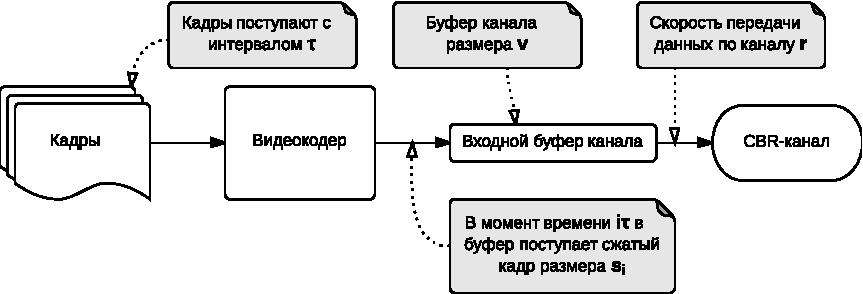
\includegraphics[width=\textwidth]{delay_jitter_model.pdf}
    \end{center}
    \caption{Модель системы передачи видеотрафика для исследования
    характеристик качества обслуживания}
    \label{fig:delay_jitter_model}
\end{figure}

Процесс передачи данных в расматриваемой модели происходит следующим
образом: с интервалом $\tau$ в момент $\tau i$ с выхода
кодера в буфер канала объёмом $v$, в котором на данный момент
находится $k_i$ байт, поступают $s_i$ байт информации, $i = 1 \dots N$.
Если происходит переполнение буфера, излишек считается утерянным.
Содержимое буфера передаётся по каналу с фиксированной скоростью
$v$. Если буфер оказывается пустым, канал ожидает поступления
новых данных, после чего возобновляет передачу.
Эта модель значительно проще реальных систем передачи данных
и исходит из следующих допущений:

\begin{itemize}
    \item видеокодер способен обеспечивать стабильный период следования кадров $\tau = const$;
    \item используется канал с постоянной битовой скоростью;
    \item не учитываются добавочные нагрузки на передачу заголовков пакетов
        и прочей служебной информации;
    \item не рассматривается буферизация на стороне получателя и вопросы начальной буферизации;
    \item не предпринимается попыток восстановления данных при переполнении
        буфера отправителя.
\end{itemize}

Приведённые допущения оправданы в силу того, что полноценное моделирование
канала передачи информации не приведёт к более достоверному сравнению
моделей видеотрафика, значительно усложнив при этом задачу моделирования канала.


\subsubsection{Коэффициент потерь при переполнении буфера}
\hspace{3pt}

Исследование коэффициента потери при предачи по каналу
с фиксироованным буфером на входе (``тест с текущим ведром'',
англ. Leaky-Bucket Test) является основным
методом исследования неравномерности трафика (burstiness),
применявшимся с первых исследований передачи VBR-трафика
\cite{}.
Коэффициент потери ячеек (англ. Cell Loss Rate) являлся
важнейшей характеристикой качества обслуживания при передаче
данных по сети ATM.

Пусть есть канал с фиксированной постоянной пропускной
способностью $r$, на входе которого стоит буфер размера $v$.
На вход канала с постоянной частотой поступают сжатые
кадры. Далее приведено пошаговое описание теста, осуществляемого
при помощи имитационного моделирования описанного канала.

За шаг времени $\tau$ примем интервал между поступлениями
кадров. Пусть на момент поступления очередного кадра размера
$s_i$ в буфере осталось $k \in [0; v]$ непереданных байт.
В случае, если текущий не может быть сохранён
в буфере ($ns_i = s_i + k > v$), буфер переполняется и излишек $o_i = ns_i - v$
считается потерянным. К появлению следующего кадра
в буфере останется $k \leftarrow \max(\min(ns, v) - r\tau, 0)$ байт,
после чего процедура повторяется для следующего кадра.
Контроль целостности кадров в данном тесте не осуществляется.

Метрикой каждой последовательности размеров кадров будем считать
долю потерянных байтов к общему объёму передаваемых данных
в последовательности:

\begin{equation}
    \eta = \frac{\sum_i o_i}{\sum_i s_i},
\end{equation}
суммирование ведётся по входящей последовательности кадров.

Расмотренная модель канала параметризуется двумя параметрами:
размером буфера $v$ и пропускной способностью на кадр $r\tau$.
Для получения релевантных результатов теста необходимо правильно
подбирать эти параметры в зависимости от статистических параметров
входной последовательности. Для определения области допустимых значений
необходимо рассмотреть данный канал как систему массового обслуживания
\cite{}
(СМО). В соответствии с расширенной нотацией Кендалла
\cite{},
данная модель имеет тип D/G/1/$v$, то есть распределение
вероятностей поступления заявок в систему детерминировано
(заявки поступают с интервалом $\tau^{-1}$), распределение
времени обслуживания произвольно и зависит от распределения
размеров кадров, очередь обслуживает один обработчик,
а объём очереди равен $v$. Существенно, что размер очереди
определяется не количеством слотов, а объёмом невыполненной
работы в очереди, в полным соответствии с аналогией ``текущего
ведра''.

Рассмотрение приведённой модели канала в качестве СМО позволяет
сформулировать граничные условия применимости данной модели
канала при сравнении различных моделей видеопоследовательностей:
в соответствии с условием стационарности СМО, интенсивность
входного потока заявок не должна превышать интенсивность обслуживания
\cite{},
следовательно

\begin{equation}
    \frac{\lambda}{\mu} = \frac{\overline{s}}{r\tau} \ < 1,
\end{equation}
интенсивность входного потока равна $\overline{s}/\tau$ байт/сек
(предполагается стационарность входного потока),
интенсивность обслуживания равна $r$ байт/сек по определению.
Таким образом, для обеспечения стационарного режима работы необходимо
установить пропускную способность канала большей, чем средний размер
кадра. Для установленной пропускной способности канала и для различных
последовательностей размеров кадров варьируется размер буфера в некотором
диапазоне от среднего размера кадров, полученные зависимости
сравниваются между собой.

\subsubsection{Задержка в получении кадра и джиттер}
\hspace{3pt}

В настоящее время мультимедиа данные, в том числе и трафик видеоконференций,
передаются преимущественно по IP-сетям, важнейшими критериями качества обслуживания
для которых
являются задержка в получении пакета (англ. delay) и джиттер, или дрожание
(англ. jitter), то есть отклонение в интервале поступления пакетов.

В целях сравнительного анализа моделей видеотрафика на основе задержки
и джиттера предлагается рассматривать модель канала, схожую с рассмотренной
при анализе коэффициента потерь, но с неограниченным буфером на входе.

В рамках данного теста передача осуществляется без потерь. В момент времени
$\tau i$ кадр под номером $i$ приходит в систему и заполняет $s_i$
байт в буфере. Канал передаёт содержимое буфера с постоянной скоростью
$r$ и в некоторый момент времени $t_i$ закончит передавать последний
байт кадра $i$. Промежуток времени между поступлением кадра в систему и полной
передачей кадра в канал $d_i = t_i - \tau i$ называется задержкой
и может рассматриваться как случайная величина, зависящая от
входного потока кадров и от пропускной способности канала $r$.

Джиттер характеризует степень неустойчивости интервалов появления
кадров на принимающей стороне канала. В некоторых источниках
\cite{}
джиттером называют дисперсию задержки, в других
\cite{}
--- производную задержки по времени. В работе используется
второе определение, так как оценка джиттера таким способом
используется на приёмной стороне, для которой данные о поступлении
кадров в систему недоступны.

Совокупность промежутков между получением двух соседних кадров $t_{i+1} - t_i$
называется джиттером и может быть получена на основе задержки следующим образом:

\begin{equation}
    \left\{
    \begin{aligned}
        d_i &= t_i - \tau i\\
        d_{i+1} &= t_{i+1} - \tau (i+1),\\
    \end{aligned}
    \right.
\end{equation}
\begin{equation}
    \begin{aligned}
    d_{i+1} - d_i &= t_{i+1} - \tau i - \tau - t_i + \tau i\\
                  &= t_{i+1} - t_i - \tau\\
    \Longrightarrow t_{i+1} - t_i &= d_{i+1} - d_i + \tau
    \end{aligned}
\end{equation}

Рассуждения, аналогичные приведённым при рассмотрении коэффициента
потерь для определения граничной пропускной способности канала,
применимы и при оценке задержки и джиттера.

Моделирование канала для получения значений задержек было
осуществлено при помощи двух методик имитационного моделирования:
дискретно-событийного моделирования и аналитического метода.
Далее приведено описание обеих методик.

В рамках дискретно-событийного моделирования временная шкала
разбивается на кванты времени длительностью $q$. В качестве 
параметров модели указывается количество квантов времени в
периоде следования кадров и количество байт, передаваемых
каналом за квант времени $b$. Непереданный остаток от текущего
кадра и его индекс хранятся в переменных. На каждом шаге
алгоритма происходит уменьшение остатка от текущего кадра
на $b$ байт. После того, как текущий кадр передан целиком
(остаток стал меньшим либо равным нулю), в качестве задержки
для текущего кадра сохраняется разность текущего времени со
временем поступления кадра $i \tau$ (может быть вычислено аналитически в любой момент).
Далее, в случае, если время появления следующего кадра в системе
ещё не наступило (буфер опустел), программа инкрементирует
счётчик времени до прихода следующего кадра. Если же следующий
кадр уже пребывает в системе, моделирующая программа принимает
этот кадр за текущий и повторяет описанную процедуру.

Данный подход имеет ряд преимуществ: с его помощью удаётся
избежать явного отслеживания состояния буфера,
он максимально точно отражает логику передачи данных в реальном
канале с буфером и потенциально данный подход можно
без особых изменений применить и для канала с переменной
битовой скоростью, как и для случая неравномерного поступления
кадров в буфер или для более сложных политик передачи данных
(очередь с приоритетами и пр.). Однако в рамках данного подхода приходится
учитывать пограничные случаи, такие как возможность при
непустом буфере в рамках одного кванта передавать
данные от нескольких кадров. Кроме того, данный подход вынуждает
использующего моделирующую программу в явном виде указывать
ненужные с точки зрения анализа моделей параметры, такие,
как количество квант на кадр.

Вышеизложенные соображения позволяют сделать вывод об
избыточности дискретно-событийного метода имитационного
моделирования в рамках задачи нахождения задержки
и джиттера в канале с постоянной пропускной способностью.
В связи с этим был предложен альтернативный метод
моделирования, в большей степени полагающийся на
заданные свойства системы (равномерное поступление
кадров на вход, CBR-канал) и потому более простой
в реализации.

За один такт модели примем поступление очередного
$i$-го кадра в систему. Пусть на этот момент в
буфере отправителя находится $b_i$ байт информации,
пропускная способность равна $r\tau$ байт на кадр.
Текущий кадр будет передан после того, как будет
передано содержимое буфера, поэтому время передачи
текущего кадра вычисляется следующим образом:

\begin{equation}
    d_i = \frac{s_i + b_i}{r\tau}.
\end{equation}

К моменту поступления следующего кадра в буфере
останется $b_{i+1} = \max(s_i + b_i - r\tau, 0)$
байт. Это значение принимается за текущее состояние
буфера и алгоритм переходит к следующему кадру.

Помимо простоты данного подхода следует отметить и
тот факт, что результирующая задержка не дискретизована
до размера кванта, поэтому данный метод демонстрирует
большую точность при большей производительности.
Результаты моделирования обоими способами совпадают
с точностью до размера кванта в дискретно-событийной модели.
В ходе сравнения различных моделей видеотрафика использовался
аналитический метод моделирования канала.

Полученные последовательности задержек $d_i$ и интервалов
между появлениями кадра на получателе $\Delta t_i$, $i = 1 \dots N$
рассматриваются как выборки случайной величины, для которой
могут быть получены стандартные статистические характеристики.
Именно математические ожидания задержки и джиттера выбраны
в данной работе в качестве характеристик
конкретной модели при фиксированных параметрах канала.

\section{Результаты сравнительного анализа моделей}
\label{sec:results}

\subsection{Сравнение гистограмм}
\label{sub:histresults}

Типовая гистограмма представлена на рисунке~\ref{fig:romanCapShisto}.
Дискретная авторегрессионная модель с отрицательным биномиальным
распределением в качестве остаточного (см. подраздел~\ref{sse:darp})
хорошо отражает моделируемый тип трафика. Марковские модели
в силу ограниченного количества квантов (здесь и далее представлены
реализации марковских моделей с двадцатью состояниями)
характеризуются импульсным характером функции распределения.
Нормированность гистограммы и провалы в отрезках, не содержащих
аппроксимирующих значений, приводят к увеличению значений
оценки функции плотности вероятностей относительно гистограммы
исходной последовательности.

Гистограммы на рисунке~\ref{fig:romanCapShisto} не демонстрируют
очевидного преимущества использования неравномерного квантования
(подраздел~\ref{sse:markkmeans}) перед равномерным (подраздел~\ref{sse:marksimple}).
Однако в случае распределения с ``длинным хвостом'' ситуация в корне меняется.
На рисунке~\ref{fig:borisFullMKhisto} представлено сравнение гистограмм
для тестового видео с ``длинным хвостом'' распределения
и для марковской модели с нелинейным квантованием (MK).
Видно, что почти все аппроксимирующие
значения находятся в области ``купола'' распределения, или
в области концентрации энергии последовательности.
На следующем
наборе гистограмм (рисунок~\ref{fig:borisFullMLhisto})
для той же видеопоследовательности дополнительно приведена
гистограмма для простой цепи Маркова с равномерным квантованием.
Так как в рамках этой модели область значений размеров кадров
разбивается на равные отрезки, на область ``купола'' пришлось
всего три состояния, а для набора статистики переходов в область
``хвоста'' просто не хватило данных.

В целом, сравнение гистограмм распределений размеров кадров
показывает, что нелинейная марковская модель лучше отражает
распределение размеров кадров тестовых последовательностей.
В то же время, аппроксимация распределения обратным биномиальным
распределением тоже достаточно точна.

\subsection{Сравнение функций автокорреляции}

Сравнение функций автокорреляции (англ. ACF) целесообразно осуществлять
отдельно при маленьких при больших значениях сдвига
для анализа краткосрочной и долгосрочной зависимостей.

Сравнение ACF для краткосрочных зависимостей на рисунке~\ref{fig:akiyosrd}
показывает, что для тестового видео Akiyo предложенная модель с
нелинейным квантованием лучше других соответствует исходной
последовательности. В целом, все предложенные модели достаточно
точно отражают краткосрочные зависимости в трафике видеоконференций.

Анализ долгосрочных зависимостей (рисунок~\ref{fig:borisFullacflong})
показывает, что в некоторых случаях предложенные модели
успешно отражают и долгосрочные зависимости. Однако
для тестовых последовательностей высокого качества в целом
характерна неспособность отразить субэкспоненциальное
убывание автокорреляции, продемонстрированное на рисунке~\ref{fig:romanCpamMacf}.

\subsection{Сравнение характеристик качества обслуживания}

Анализ характеристик качества обслуживания может давать
дополнительные сведения о применимости той или иной
модели для данного тестового видео. Так, на рисунке~\ref{fig:borisFullbucket}
приведено сравнение коэффикиента потери при переполнении буфера
в рамках теста с текущим ведром (описан в подразделе~\ref{sse:bucket}).
Тест позволяет сделать вывод об адекватности использования
марковской нелинейной модели для этого видео. При этом
марковская линейная модель (ML) демонстрирует худший результат
на этом тесте.

Анализ задержки в некоторых случаях может давать ценную информацию
о качестве модели. Так, в случае с тестовым видео Akiyo (рисунок~\ref{fig:akiyodelaypresentation})
лучше всего по критерию задержки исходному трейсу соответствует дискретная
авторегрессионная модель второго порядка. Марковская нелинейная модель и на этом
тесте превосходит линейную. В некоторых случаях анализ задержки выявляет
неспособность используемых моделей отражать тестовые видео, в особенности
видео высокого качества с ``длинным хвостом''. Представленная на рисунке~\ref{fig:borisFulldelay}
ситуация является следствием серии из больших значений в моделируемом трейсе,
в результате которой буфер отправителя единовременно заполняется большим объёмом данных,
что вызывает лавинообразный рост задержки при передаче последующих кадров и сказывается на среднем
значении этой величины при любой пропускной способности канала.

Сравнение среднего джиттера для разных моделей (рисунок~\ref{fig:akiyojitter})
в некоторых случаях позволяет признать неадекватными некоторые модели.
Так, в случае с последовательностью Akiyo исследование джиттера побуждает
отказаться от моделирования этого видео с помощью модели DAR(1) и линейной
марковской модели.

\subsection{Результаты сравнения моделей}

Сравнительный анализ моделей позволяет прийти к следующим заключениям:

\begin{itemize}
    \item Выбранные модели хорошо отражают краткосрочные
        зависимости в моделируемом трафике
    \item Предложенная марковская модель с нелинейным квантованием
        превосходит линейную модель для б\'{о}льшей части
        тестовых видеопоследовательностей
    \item Предлложенная оценка задержки и джиттера является
        полезным дополнением к имеющимся методикам сравнительного анализа моделей
    \item Тестовые видео хорошего качества обладают
        долгосрочными зависимостями
    \item Предложенные модели ``работают'' для тестовых
        видео плохого качества, но не способны отражать
        долгосрочные зависимости качественных видеопоследовательностей
\end{itemize}

    \begin{figure}[h]
        \begin{center}
            \includegraphics[width=\textwidth]{romanCapS_histo.pdf}
        \end{center}
        \caption{Сравнение гистограмм размеров кадров для различных моделей (RomanS)}
        \label{fig:romanCapShisto}
    \end{figure}

    \begin{figure}[h]
        \begin{center}
            \includegraphics[width=\textwidth]{borisFullMK_histo.pdf}
        \end{center}
        \caption{Сравнение гистограмм размеров кадров для различных моделей (Boris)}
        \label{fig:borisFullMKhisto}
    \end{figure}

    \begin{figure}[h]
        \begin{center}
            \includegraphics[width=\textwidth]{borisFullML_histo.pdf}
        \end{center}
        \caption{Сравнение гистограмм размеров кадров для различных моделей (Boris)}
        \label{fig:borisFullMLhisto}
    \end{figure}

    \begin{figure}[h]
        \begin{center}
            \includegraphics[width=\textwidth]{akiyo_srd.pdf}
        \end{center}
        \caption{Сравнение автокорреляции для различных моделей (SRD) (akiyo)}
        \label{fig:akiyosrd}
    \end{figure}

    \begin{figure}[h]
        \begin{center}
            \includegraphics[width=\textwidth]{borisFull_acflong.pdf}
        \end{center}
        \caption{Сравнение автокорреляции для различных моделей (LRD) (Boris)}
        \label{fig:borisFullacflong}
    \end{figure}

    \begin{figure}[h]
        \begin{center}
            \includegraphics[width=\textwidth]{romanCapM_acf.pdf}
        \end{center}
        \caption{Сравнение автокорреляции для различных моделей (LRD) (RomanM)}
        \label{fig:romanCpamMacf}
    \end{figure}

    \begin{figure}[h]
        \begin{center}
            \includegraphics[width=\textwidth]{borisFull_bucket.pdf}
        \end{center}
        \caption{Тест с текущим ведром (Boris)}
        \label{fig:borisFullbucket}
    \end{figure}

    \begin{figure}[h]
        \begin{center}
            \includegraphics[width=\textwidth]{akiyo_delay_presentation.pdf}
        \end{center}
        \caption{Задержка при передаче по CBR-каналу (akiyo)}
        \label{fig:akiyodelaypresentation}
    \end{figure}

    \begin{figure}[h]
        \begin{center}
            \includegraphics[width=\textwidth]{borisFull_delay.pdf}
        \end{center}
        \caption{Задержка при передаче по CBR-каналу (Boris)}
        \label{fig:borisFulldelay}
    \end{figure}

    \begin{figure}[h]
        \begin{center}
            \includegraphics[width=\textwidth]{akiyo_jitter.pdf}
        \end{center}
        \caption{Джиттер при передаче по CBR-каналу (akiyo)}
        \label{fig:akiyojitter}
    \end{figure}


\sectioncentered*{Заключение}
\addcontentsline{toc}{section}{Заключение}

В данной дипломной работе была рассмотрена задача моделирования трафика видеоконференций,
сжатого с помощью видеокодера с переменной битовой скоростью.
Были исследованы существующие подходы к моделированию видеотрафика с переменной
битовой скоростью (раздел~\ref{sec:survey}) и выбраны подходы и конкретные модели, в наибольшей степени
подходящие для моделирования трафика видеоконференций.

Были реализованы две из существующих моделей: дискретная авторегрессионная модель
произвольного порядка DAR(p) (модель порядка более высокого, чем DAR(1), в литературе
не встречалась) и марковская модель на основе марковского возобновляемого процесса
(MRP). Для марковской модели была предложена модификация,
демонстрирующая лучшие результаты при сравнительном анализе (раздел~\ref{sec:models_description}).

Исследованы использующиеся методы сравнительного анализа моделей на основе
статистических характеристик и на основе коэффициента потерь при
переполнении буфера при передаче по сети с постоянной битовой
скоростью (раздел~\ref{sec:comparision}). Эти и предложенные автором методы были применены для анализа
адекватности моделей в имитировании видеопоследовательностей тестового
множества.

Была предложена методика сравнительного анализа моделей на основе
задержки и джиттера, предоставляющая дополнительную информацию
об адекватности модели. Использование этих характеристик
качества обслуживания уже предлагалось в литературе~\cite{survey2013}, но
на практике задержка и джиттер не использовались таким образом.

Сравнительный анализ моделей (раздел~\ref{sec:results}) показал адекватность использования
выбранных моделей для имитации трафика видеоконференций плохого
и среднего качества, однако выявил долгосрочные зависимости в видеоконференциях
хорошего качества и неспособность реализованных моделей их
отражать. Наличие долгосрочных зависимостей в трафике данного типа
не обнаружено в исследовательских работах~\cite{survey2013, ars2004, characteristics2013},
что позволяет говорить о необходимости в дополнительном исследовании
моделирования трафика HD-видеоконференций.



\input{references}

% \includepdf позволяет включить в результирующий pdf документ часть другого pdf документа, сделанного
% например не с помощью TeX. Бывает полезно, если какие-то диаграммны нарисованы, например, с помощью 
% Microoft Office и сохранены в pdf.
%\includepdf[pages={-}]{documents_list.pdf}

\end{document}
